%-----------------------------------------------------------------------------------------------
\chapter{Quad detection}\label{sect:quad_detection}
%-----------------------------------------------------------------------------------------------

In this chapter there will be a summary of the image processing algorithms tried and used for the recognition of the fiducial markers.
The input of this recognition step is the image taken by the camera, and the output is a list of quads belonging to the marker visible on the image.
As a common preprocessing step for all quad detection methods segmentation is performed on the input image: quad-like blobs are extracted and separately passed to the quad detector logic.
This step of the \textit{marker recognition process} takes the segmented input image and initialises quad structures based on the observed picture.
The quad structures are then passed to the next processing step: the pose estimation logic.

The process here diverges depending on which quad detection algorithm is used.
They all need differently conditioned input images for optimal performance.
From a computer vision point of view the task is to detect joint line segments.
This is a well researched task in image processing, there are many well tried algorithms for it.
For example, the problem can be solved by detecting lines and finding their intersection, or detecting corners and figuring out how they are connected, etc...
The detection routines not necessarily have the same output format\footnote{Some return line segments defined by their endpoint, others use the polar representation of a line etc.}, so conversion may also be needed.

Three separate quad detection techniques and their variants were profiled in this experiment.
\begin{itemize}
	\item Hough-transformation
	\item Corner detection
	\item Line Segment Detector\cite{LSDDet}
\end{itemize}
The first one uses the Hough-transformation for line detection.
There are many variants of the transformation: Standard Hough Transform, Probabilistic Hough Transform, Multiscale Hough Transform, etc...
The 2 most commonly used are the standard- and the probabilistic variants.
The OpenCV framework offers implementations for them, both were tested in the experiment.

The second detector is based on corner recognition.
There are more variants of this method to try out, too.
The corner metrics of a feature can be calculated differently with (Harris metric, eigenvalues, etc.) varying results.
It is also needed for the solution to be scale invariant, which also can be achieved in a number of ways.

The third alternative is the Line Segment Detector algorithm described in \cite{LSDDet}.
It is a robust and fast algorithm for detecting line segments on an image.
The OpenCV framework provides an implementation of it as well.

A typical marker shot with partial visibility is shown figure \figref{partialMarkerShot}.
\begin{figure}[ht]
	\centering
	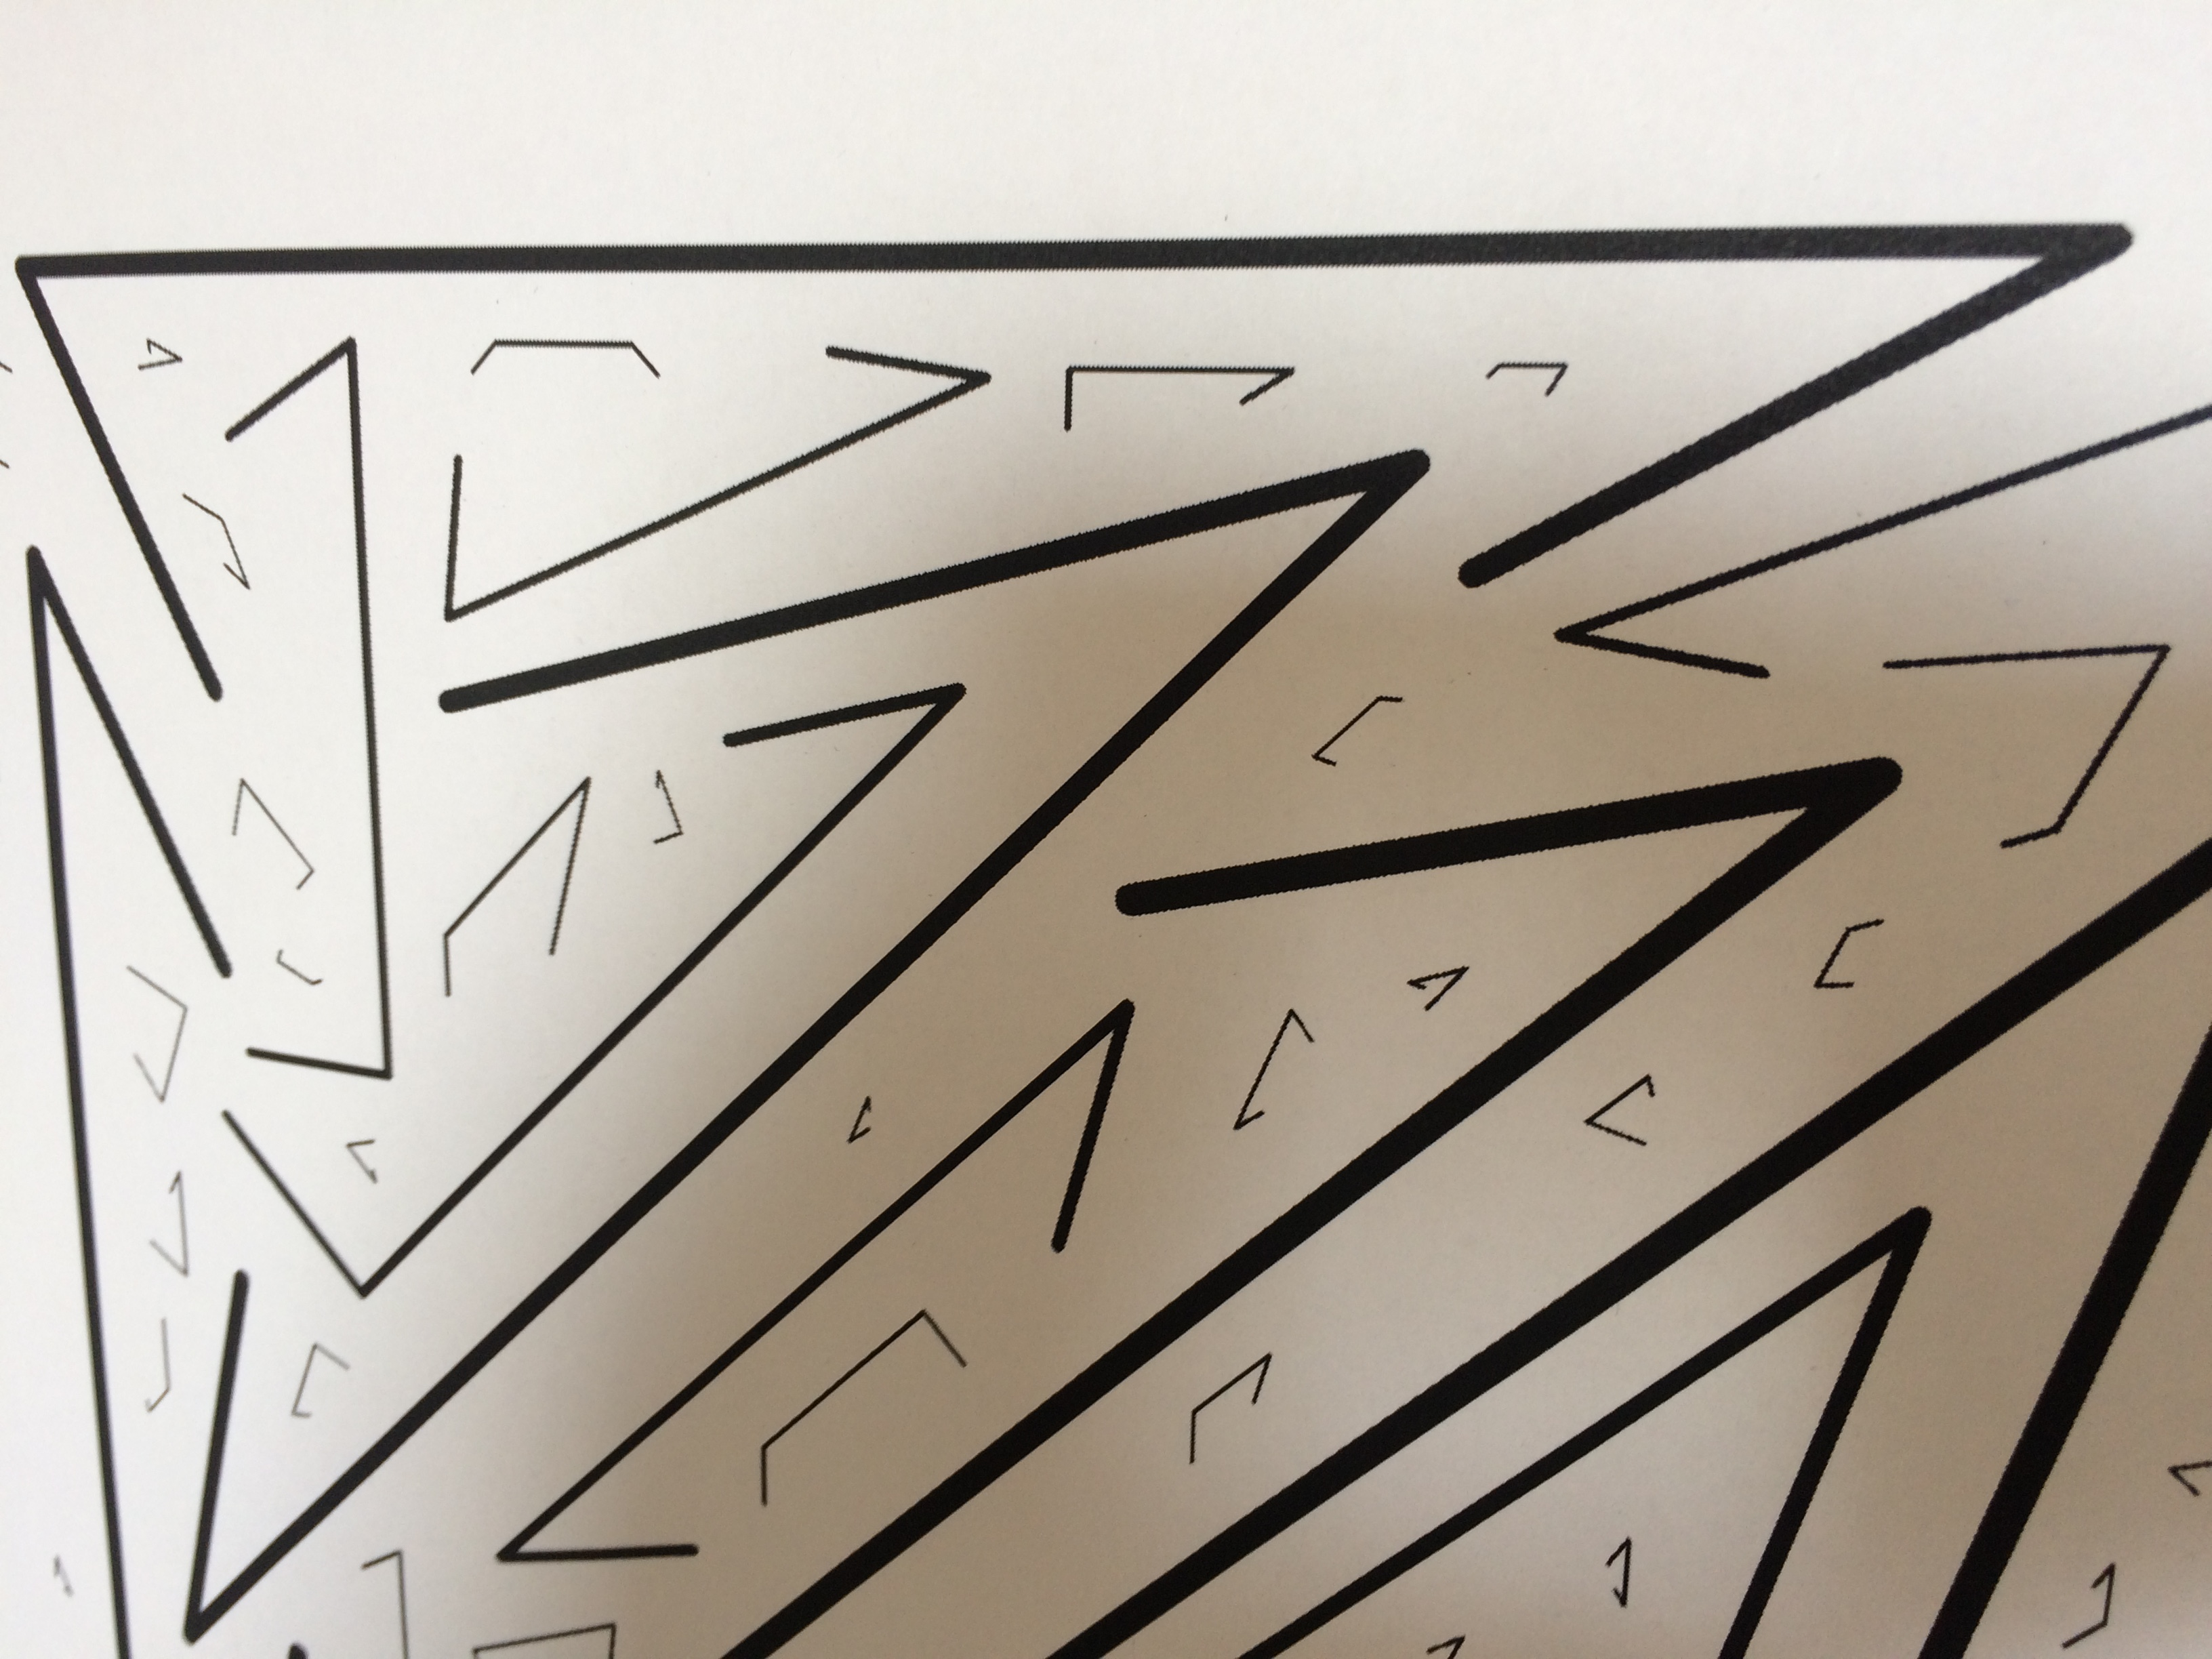
\includegraphics[width=0.75\textwidth]{figures/t35_01.JPG}
	\caption{Partially visible marker (taken with commercial smartphone)}
	\label{fig:partialMarkerShot}
\end{figure}
In this chapter will be a short summary of the algorithms used for testing and performance comparison.

%-----------------------------------------------------------------------------------------------
\section{Theoretical Overview}
%-----------------------------------------------------------------------------------------------

Before going over how the image processing algorithms were applied to achieve quad detection, a short theoretical overview of the used algorithms will be presented.
To solve the problem at hand (i.e. to detect quad instances on an image) multiple well known image processing algorithms were used.
For line detection two variants of the Hough transform (Standard\cite{houghThetaRho} and Probabilistic\cite{MATAS2000119}) and a fundamentally different algorithm, the \textbf{LSD} was used.
As mentioned before, not only solutions based on line detection were tried during the course of this work; corner detection methods were also tried.
The Harris corner detector\cite{Harris88alvey} and it's improved version the Shi-Tomasi detector\cite{Shi94goodfeatures} were compared.

Although the implementation of the aforementioned algorithms were provided by the OpenCV framework, it was far from unnecessary to understand how each algorithm works.
They show their optimal performance on differently conditioned inputs.
For example, corner detection works well on "raw" images, while the Hough-transform based solutions need edge images of skeletons to perform.
It was important to know the limitations of each solution.
All in all, the understanding of the inner workings of the algorithms used was helpful in choosing the "right tool for the job".

In this section there will be the theoretical overview of the above mentioned algorithms, with some historical context.
Their comparative advantages for this project will also be highlighted.

%-----------------------------------------------------------------------------------------------
\subsection{Hough transformation}
%-----------------------------------------------------------------------------------------------

One of the most commonly used methods for line detection on images is the Hough transform.
Over it's long history many publications have been made about it's applications, performance and improvements.

Originally it was developed by Paul Hough in 1959 and later patented in 1962\cite{houghPatent}.
It was intended to be used for machine analysis of bubble chamber photographs.
In it's modern form (with the $\theta-\rho$ parametrisation) was introduced in 1972 by Duda and Hart\cite{houghThetaRho}.
The transformation became popular in the image processing community after Ballard's article\cite{BALLARD1981111} about generalising the algorithm for detection of arbitrary shapes.
There were many optimised and improved variants of the transformation, however the basic concept remained the same.
In 1990 a publication\cite{XU1990331} introduced the Randomized Hough Transform, which was a fundamentally new approach to the algorithm with notable merits.
As opposed to the one-to-many mapping of the simple Hough transform, the randomised version uses a convergent many-to-one mapping when creating the parameter space.

In this work the Standard Hough Transform and one of it's optimised versions, the Progressive Probabilistic Hough Transform will be used.
The PPHT, although being probabilistic, doesn't belong to the class of randomised Hough transforms.
It uses the same one-to-many mapping as the SHT.
The OpenCV framework provides implementations for the SHT and the PPHT, which is one of the main reason why they were chosen for this project.

After this short historical overview the theory of the transformations will be discussed.

%-----------------------------------------------------------------------------------------------
\subsubsection{Standard Hough Transform}
%-----------------------------------------------------------------------------------------------

The transformation is used to find instances of a model on digital images.
The models are usually simple geometric shapes like lines, circles or ellipses.
The curves are described by their parameters, e.g. slope and intercept for a line, centre point and radius for a circle etc..
Every non-zero pixel\footnote{The transformation works on binary images} votes for the features it could be part of.
The number of votes is stored for every possible parameter combination.
Then a threshold is applied to the stored votes, and the remaining parameters are accepted as model instances.
	
At first Hough described the algorithm to lines, but later the method would be generalised to any analytic\footnote{The Generalised Hough Transform even extends to arbitrary shapes} curve or shape.
This theoretical overview is based on the example of line detection.
The process is the same for every analytic curve, the only difference is the parameter space's dimension.
The original patent\cite{houghPatent} used the slope-intercept representation of lines.
\begin{equation}
y = m*x + b
\end{equation}
In this case, the \emph{parameter space} is 2 dimensional and it's axes are $m$ and $b$.
Every point in the parameter space represent an image space line.
With this representation every non-zero pixel in the image space transforms into a line in the parameter space.
For a given $(x_0,y_0)$ pair \eqref{houghLineMB} gives the line in the parameter space. 
\begin{equation}
\label{eq:houghLineMB}
b = -x_0*m + y_0
\end{equation}
Collinear points in the image show up in the parameter space as intersecting lines.
The more lines intersect in a given $(m_0,b_0)$, the more likely it is the image contains the $y = m_0*x + b_0$ line.
The problem with this parametrisation is that the parameter space is unbounded along both axes.
Both intersect and slope can have values in the range of $(-\infty, \infty)$.
Duda and Hart\cite{houghThetaRho} proposed an alternative parametrisation, which turned out to be better for application.
They used the \emph{normal parametrisation} of a line, shown in \eqref{normalParams}.
\begin{equation}
	\label{eq:normalParams}
	\rho = x*cos(\theta) + y*sin(\theta)
\end{equation}
In \eqref{normalParams} $\rho$ means the distance of the line from the image plane's origin.
$\theta$ is angle of the normal vector of the line.
\begin{figure}[ht]
	\centering
	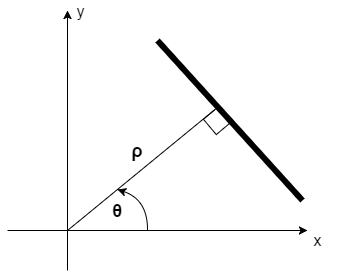
\includegraphics[width=0.5\textwidth]{figures/line_params.png}
	\caption{Normal line parameters}
	\label{fig:normalLineParams}
\end{figure}
If the \emph{normal parametrisation} is used the parameter space becomes finite in both dimensions.
$\theta$ is in the range of $(0,2\pi)$, $\rho$ is bounded by the image size.
In this case the image points define sinusoid curves in the parameter plane, and the line detection is done by searching for their intersections.
\begin{figure}[ht]
	\centering
	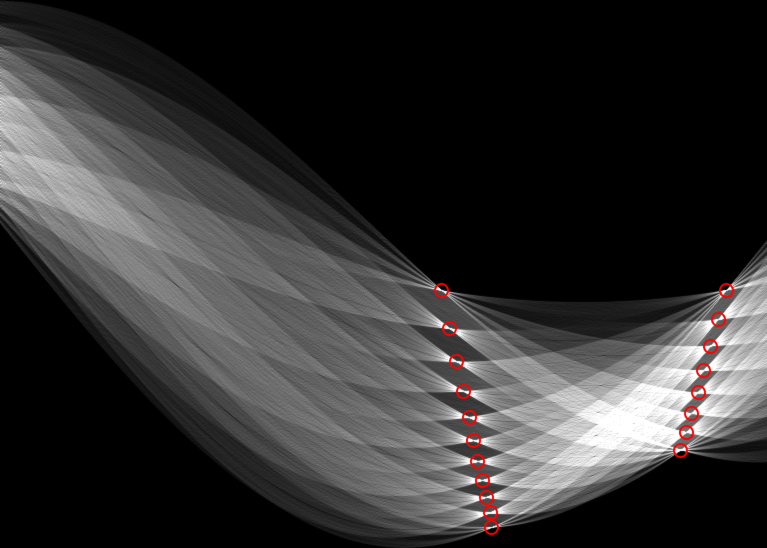
\includegraphics[width=0.6\textwidth]{figures/Perspective_chessboard_hough_transform.png}
	\caption{Hough-transform of a chessboard pattern}
	\label{fig:houghChessBoard}
\end{figure}

As mentioned before, the line detection is based on a voting scheme.
The parameter space (in this case a 2 dimensional plane) is divided into \emph{bins}.
$\rho$ and $\theta$ are quantised in the desired resolution.
The discrete $(\rho,\theta)$ pairs define the bins.
Every bin has accumulator.
When a given $(\rho_i,\theta_i)$ pair gets a vote it's corresponding accumulator is incremented by 1.
The \textbf{SHT} (Standard Hough Transform) uses one-to-many divergent mapping.
This means that every non-zero pixel votes for every possible parameter pair it could belong to.
The above mentioned sinusoid is calculated with the desired resolution for the pixel, and the corresponding accumulators are updated.

When the accumulation phase is completed for the whole image, the local maxima of the accumulators are found.
Usually a threshold is applied in order to reduce noise and eliminate too short line segments.
The radius of the non-maxima suppression also has impact on the results of the line fitting, it must be chosen carefully.
After this step the parameters for the most likely line candidates are available.

As the \textbf{SHT} does not provide the endpoints of the line, they must be found by examining the original binary image.
This can be done by simple checking every pixel along the line with the given parameters and deciding whether or not it is part of the feature.
If it is desired, lines with gaps can also be accepted with this method.
For more accurate fitting, a Least Squares approximation can also be applied to the pixels belonging to the line.

%-----------------------------------------------------------------------------------------------
\subsubsection{Progressive Probabilistic Hough Transform}
%-----------------------------------------------------------------------------------------------

The progressive probabilistic Hough transform is an optimised version of the SHT described in \cite{MATAS2000119}.
Probabilistic Hough transform variants were developed to overcome the comparatively high computational cost of the standard transform.
The core concept is the same for most probabilistic versions of the Hough transform: not every none-zero point votes, only a randomly selected subset.
These algorithms have to find a balance between minimising the proportion of image points that are used for voting while maintaining the accuracy of the detection process.

The original probabilistic Hough transform\cite{KIRYATI1991303} solved this issue by introducing a tunable parameter $p$ for the fraction of points to be used.
First, a $p$ fraction of the non-zero points are selected, than the SHT is performed on the selected subset.
$p$ can be low, the authors of \cite{KIRYATI1991303} presented successful experiments with $p=2\%$.
However, the results of the algorithm are greatly sensitive to the sampling rate.
The authors analysed the problem on the special case of a single line immersed in noise and tried to formulate a solution for determining the $p$ parameter.
They succeeded, but the practical applicability is severely limited\cite{MATAS2000119}: it requires \textit{a priori} knowledge of the number of points belonging to the line.
There was another approach to calculate the number of necessary votes\cite{BERGEN1991639}.
It was shown that the probabilistic Hough transform can be formulated as the Monte Carlo approximation of the SHT, thus it is possible to deduce the desired error rate using the theory of Monte Carlo evaluation.
Nevertheless, the core problem remained the same: \textit{a priori} information was necessary for determining the sampling rate parameter.
Usually there is only very limited information available, so conservative approximation is needed.
This leads to the calculation of more votes then necessary, thus reducing the main advantage of the probabilistic method.

The progressive probabilistic Hough transform solves the above issue by \textquote{exploiting the difference in the fraction of votes needed to reliably detect lines (features) with different number of supporting points}\cite{MATAS2000119}.
This way for long lines only a small fraction of the line's points have to vote for the line to be registered.
For shorter lines this proportion is of course higher.
For lines with supporting points close to the votes generated by background noise a full transform must be performed.

The authors of \cite{MATAS2000119} proposed the following algorithm to achieve the aforementioned goal.
At each iteration a random non-zero image point is selected for voting to the possible model instances it could belong to.
After each vote, the question \textquote{could the count be due to random noise?}\cite{MATAS2000119} is evaluated.
This requires a single comparison per bin update, with a threshold value changing by each vote cast.
When a model instance (line) is detected, the supporting points retract their votes.
The other points belonging to the same line are removed from the voting process.
The pseudo-code representation below is directly quoted from \cite{MATAS2000119}.

\begin{lstlisting}
1. Check input image, if it is empty then finish
2. Update the accumulator with a single pixel randomly selected from the 
   input image
3. Remove pixel from input image
4. Check if the highest peak in the accumulator that was modified by the 
   new pixel is higher than threshold l. If not then goto 1.
5. Look along a corridor specified by the peak in the accumulator, and find 
   the longest segment of pixels either continuous or exhibiting a gap not 
   exceeding a given threshold.
6. Remove the pixels in the segment from the input image
7. Unvote from the accumulator all the pixels from the line that have 
   previously voted.
8. If the line segment is longer than the minimum length add it into the 
   output list.
9. goto 1.
\end{lstlisting}

This algorithm has some considerable advantages of the standard and other, previous probabilistic variants of the Hough transform.
It eliminates the need of \textit{a priori} knowledge necessary for the tuning of probabilistic transforms while it remains much faster than the SHT.
It should detect every instance of a model detectable by the SHT, at the latest when the voting finishes with the same number of voted pixels as for the standard transform.
Another positive property of the algorithm is that features are detected as soon as the accumulator allows a decision: it is not necessary for all supporting points to vote.
The algorithm can also be terminated at any time and still provide some useful output\footnote{However this aspect is not really important for this project}.

Originally this transformation method was developed to speed up the Hough transform, while not being considerably more inaccurate.
However, an unexpected result was observed by the authors.
The PPHT outperformed the SHT in accuracy as well as speed.
In sample images consisting of randomly positioned equal length lines, the PPHT produced less false negatives (missed line segments) and less false positives (incorrectly detected lines).
This effect is due to the fact that PPHT clears out the votes of the detected lines as soon as they are found.
This reduces the clutter in the accumulator, resulting in more accurate results, while also being more computationally efficient.

It also worth noting that the PPHT could, in theory, use every enhancement that were developed for the SHT.
For example, the image gradient of the line segments could be used to reduce the number of pixels selected for voting.
However, this aspect was not researched in the boundaries of this project.

%-----------------------------------------------------------------------------------------------
\subsection{Line Segment Detector}
%-----------------------------------------------------------------------------------------------

A fundamentally different approach to line detection was described in \cite{LSDDet}.
The algorithm is named \textbf{LSD} - for Line Segment Detector - by it's creators.
It is which, unlike the SHT, detects line segments with subpixel accuracy by default.
The runtime of the process is linear in the pixel count of the processed image.
It also has fairly good noise suppression.
Another attractive property of the algorithm is that it doesn't have any parameters that require tuning by the user.
Every one of it's parameters are automatically tuned "under the hood".
Because of these advantageous properties was it considered for use in this project.
The implementation used was provided by the OpenCV framework.
In this section will be a short summary of the theory behind this algorithm.

The LSD takes as input a grayscale image and provides a list of line segments as output.
The line detection is based on the image gradient.
As a first step, a gradient field is generated from the input image.
The gradient is taken using a $2x2$ window, see \eqref{lsdGrad}.
\begin{equation}
	\begin{split}
		g_x = \frac{i(x+1, y) + i(x+1, y+1) - i(x,y) - i(x, y+1)}{2}, \\
		g_y = \frac{i(x, y+1) + i(x+1, y+1) - i(x,y) - i(x+1, y)}{2}
	\end{split}
	\label{eq:lsdGrad}
\end{equation}
Where $i(x,y)$ is the intensity of the grayscale image at $(x,y)$ point.
The magnitude of the gradient is calculated by \eqref{lsdGradMagn}.
\begin{equation}
	G(x,y) = \sqrt{g_x^2(x,y)+g_y^2(x,y)}
	\label{eq:lsdGradMagn}
\end{equation}
The algorithm uses the angle of the gradient, which will be referred to as LLA (level-line angle), and is calculated by \eqref{lsdGradAngle}.
\begin{equation}
	\arctan\Bigg(\frac{g_x(x,y)}{-g_y(x,y)}\Bigg)
	\label{eq:lsdGradAngle}
\end{equation}
The gradient obtained with \eqref{lsdGrad} is the image gradient at the point $(x+0.5, y+0.5)$.
This half pixel offset is later added to the endpoints of the detected line segments.

Using the gradient information, a level-line field is constructed.
\begin{figure}[ht]
	\centering
	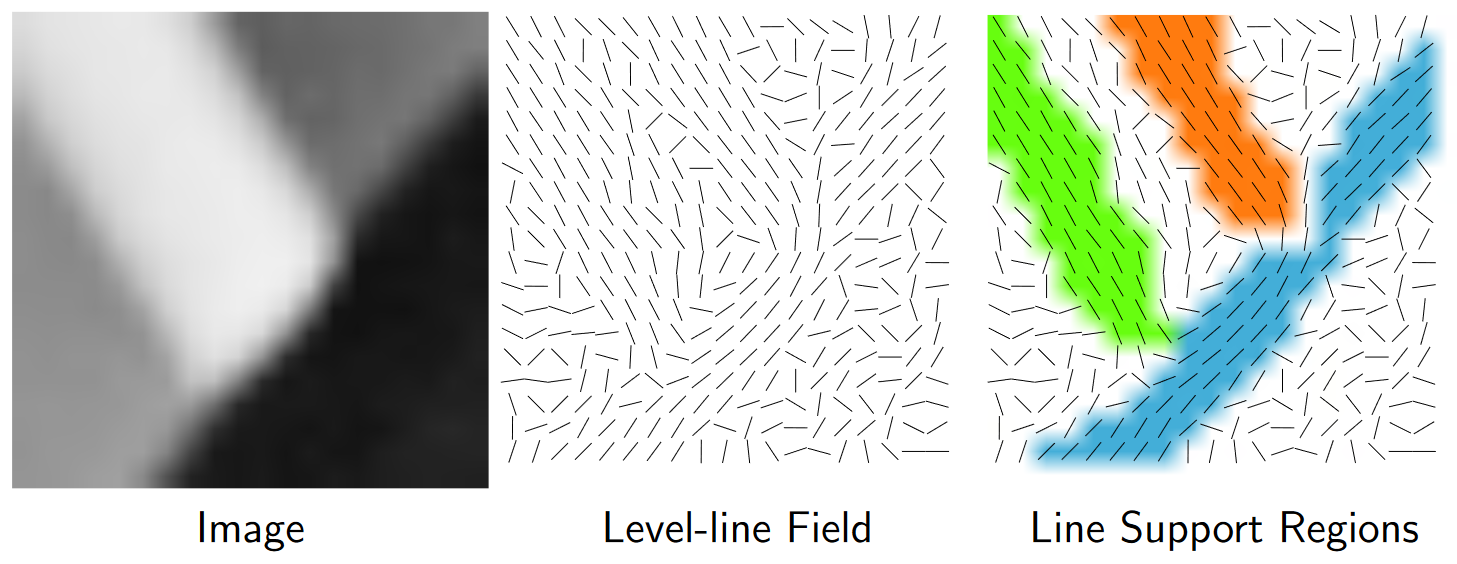
\includegraphics[width=0.75\textwidth]{figures/lsd_level_line_field.png}
	\caption{Illustration of the level-line field\cite{LSDDet}}
	\label{fig:lsdLevelLines}
\end{figure}
Figure \figref{lsdLevelLines} shows an example of the visualised level-line field.
The next step of the algorithm is the segmentation of this field.
It happens based on the level-line angle (the gradient angle defined in \eqref{lsdGradAngle}).
The pixels that have the same LLA within a given threshold are grouped together.
These segments are referred to as \textit{line support regions}, see figure \figref{lsdLevelLines} for illustration.
The segmentation is done with a region growing process.

Each \textit{line support region} is a candidate for a \textit{line segment}\cite{LSDDet}.
The line segments are represented with a rectangle.
The main direction of the rectangle is determined by the principal inertial axis of the \textit{line support region}.
The size of the rectangle is chosen in a way to cover the whole \textit{line support region}.

\begin{figure}[ht]
	\centering
	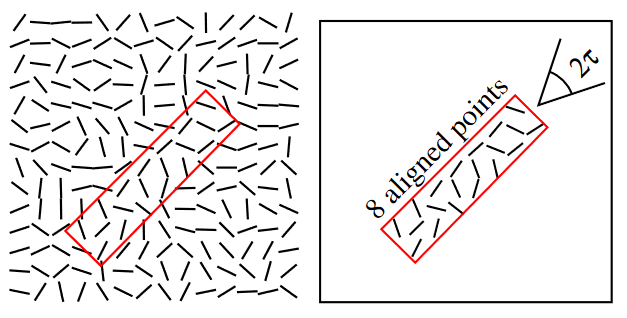
\includegraphics[width=0.75\textwidth]{figures/lsd_aligned_point.png}
	\caption{Illustration of the aligned points\cite{LSDDet}}
	\label{fig:lsdAligned}
\end{figure}
The pixels in the rectangle that have LLA close to the angle of the rectangle are called \textit{aligned points}\cite{LSDDet}.
Figure \figref{lsdAligned} shows an example for the rectangular representation and the \textit{aligned points}.
The \textit{aligned points} are used in the validation step of the algorithm.

The LSD algorithm uses an \textit{a contrario} validation method.
The idea behind that method is checking if it is probable that the current supporting points are caused by random noise.
To achieve this, the authors of \cite{LSDDet} created a noise model of the \textbf{level-line field}.
A \textit{line segment} becomes validated if the expected number of it's occurrences on the noise model is low\footnote{i.e. It is unlikely to be caused by random noise}.

The algorithm detects the sharp transients in the image gradient.
Technically, it detects edges.
A line on the image produces two line segments as output, for it's two light-dark transition.
The line segments detected by LSD are directional: the order of the endpoints of a line segments depend on the direction of the light-dark transition.

After this short summary of the algorithm\footnote{The description of the algorithm in pseudo-code form can be found in \cite{LSDDet}}, some of it's more interesting details will be described.

First off, the algorithm has a preprocessing step.
Before calculating the image gradient, the input image is downscaled to $80\%$ along both axes\footnote{or to $64\%$ of it's area}.
This is done to cope with aliasing and quantisation artefacts present in most images, for example the staircase effect.
The alternative to this subsampling would be the blurring of the image, however that would have some unfavourable side effects.
Blurring would affect the statistics of the \textit{a contrario} model.
Some structures would be detected in a blurred white noise image.
With a correct down-sampling the white noise statistics can be preserved.
The choice of scale factor was an optimum between filtering out noise and keeping valuable data.

Another interesting feature of the algorithm is the order in which the possible lines are processed.
LSD is a greedy algorithm, it tries to process the most significant edges first.
Pixels with higher gradient magnitude correspond to more contrasted edges.
In order to process the pixels with the highest contrast first, some ordering is needed.
However, most sorting algorithm require $O(n \log(n))$ operations.
To avoid this, LSD uses a pseudo ordering that can be done in linear time.
The interval between zero and the highest gradient magnitude in the image is divided into $1024$ equal bins.
Then each pixel is assigned to the bin corresponding to it's gradient magnitude.
The processing (region growing) is done first on the pixels selected from the bin containing the largest magnitudes.
$1024$ levels are enough to almost strictly order the gradients generated from a grayscale image with $256$ possible intensities.

To avoid unnecessary processing, a threshold is also applied to the gradient magnitudes.
Pixels with a low gradient represent flat regions or slowly changing intensities.
These pixels are marked and are not taking part in the later processing steps.
This threshold also helps reduce the effects of quantisation noise.	

The rectangular approximation of the line segment happens after the segmentation of the level-line field.
The rectangle is calculated based on the gradient magnitudes of the pixels belonging to a segment.
The gradient magnitude is viewed as the "mass"\cite{LSDDet} of the pixel, and the centre of the rectangle is the mass centre point of the segment.
The coordinates of the centre point are calculated by the formula given in \eqref{lsdTcpCord}
\begin{equation}
	\begin{split}
		c_x = \frac{\sum_{j \in Region} G(j) * x(j)}{\sum_{j \in Region} G(j)} \\
		c_y = \frac{\sum_{j \in Region} G(j) * y(j)}{\sum_{j \in Region} G(j)}
	\end{split}
	\label{eq:lsdTcpCord}
\end{equation}
Where $G(j)$ is the gradient magnitude of pixel $j$, calculated by \eqref{lsdGradMagn}.
$x(j)$ and $y(j)$ represent the $x$ and $y$ coordinate of point $j$, respectively.
The angle of the main rectangle is defined to be the principal inertial axis of the segment.
It can be calculated from the eigenvector of associated with the smallest eigenvalue of the matrix of \eqref{lsdMMat}.\cite{LSDDet}
\begin{equation}
	M =
	\begin{bmatrix}
		m^{xx} && m^{xy} \\
		m^{xy} && m^{yy}
	\end{bmatrix}
	\label{eq:lsdMMat}
\end{equation}
Where $m^{xx}, \dots$ is defined below.
\begin{equation}
	\begin{split}
		m^{xx} = \frac{\sum_{j \in Region} G(j) * (x(j) - c_x)^2}{\sum_{j \in Region} G(j)} \\
		m^{yy} = \frac{\sum_{j \in Region} G(j) * (y(j) - c_y)^2}{\sum_{j \in Region} G(j)} \\
		m^{xy} = \frac{\sum_{j \in Region} G(j) * (x(j) - c_x)(y(j) - c_y)}{\sum_{j \in Region} G(j)}
	\end{split}
\end{equation}

This is the short overview of the LSD algorithm, with some of it's more interesting nuances highlighted.
The full description is available in \cite{LSDDet}.

%-----------------------------------------------------------------------------------------------
\subsection{Corner Detection}
%-----------------------------------------------------------------------------------------------

Detecting quads not necessarily means the detection of line segments.
Along with the above described methods based on line detection, a corner detecting algorithm was also benchmarked.
The concept of this detection method is as follows.
Detect the corners and end-points of a quad with some corner detection algorithm.
Checks which detected pairs are connected with lines (or edges).
Based on the connected pairs and their ordering, a quad can be reconstructed.

The OpenCV framework provides implementations for some popular corner detection algorithms.
Specifically the Harris detector and the Shi-Thomas detector are covered.
In this section will be a short theoretical summary of corner detection in general, and some specifics of the above mentioned solutions.

The basic idea of most corner detection algorithm is the following.
Considering a local window on an image, corner regions show large change in average intensity if the window is shifted by a small amount in any direction.
The mathematical formulation of the following idea is shown in \eqref{moravec}.
$E_{x,y}$ is the change in intensity produced by shifting the window by $(x,y)$.
$I_{u,v}$ is the intensity of the image at the point $(u,v)$, and $w_{u,v}$ specifies the image window.
In the simplest case, the image window is rectangular and it is unity in a specified region and zero otherwise.

% Moravec corner measure
\begin{equation}
	E_{x,y} = \sum_{u,v} w_{u,v} | I_{x+u,y+v}-I_{u,v} |^2
	\label{eq:moravec}
\end{equation}

A naive approach of corner detection is to use \eqref{moravec} as it is.
The local maxima of the minimum of \eqref{moravec} above a certain threshold can be used for a metric.
With this method, three cases have to be considered:
\begin{enumerate}
	\item \textbf{Flat region:} The windowed image region has almost constant intensity. In that case, all shifts will show small change.
	\item \textbf{Edge region:} The windowed image region has an edge in it. In that case shift in one direction will result in large change, but shifts in other directions will show low change in intensity.
	\item \textbf{Corner region:} If the windowed region contains a corner, all shifts will show large change in the intensity.
\end{enumerate}

The shifts can be chosen in a couple of ways: $90^\circ$ shifts, $45^\circ$ shifts in 8 or 4 directions, etc...
Actually, this detection method is analysed in \cite{Harris88alvey}, and it is the base of the Harris detector.

\begin{figure}[t]
	\centering
	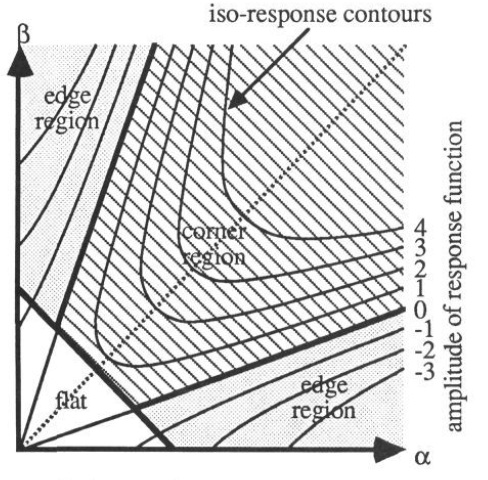
\includegraphics[width=0.75\textwidth]{figures/score-isoresponse-contours.jpg}
	\caption{Image point classification based on Harris measure\cite{Harris88alvey}}
	\label{fig:harrisMeasure}
\end{figure}

However, the the above described corner detector suffers from a number of problems\cite{Harris88alvey}.
Firstly, it provides an anisotropic response, as only a discrete set of shifts are used.
To address this issue, the Harris detector uses an analytic expansion of \eqref{moravec} around origin.
See \eqref{analyticHarris}.
\begin{equation}
	E_{x,y} = \sum_{u,v} w_{u,v} ( I_{x+u,y+v}-I_{u,v} )^2 = \sum_{u,v} w_{u,v} ( x \frac{\partial I}{\partial x} + y \frac{\partial I}{\partial y} + O(x^2,y^2))^2
	\label{eq:analyticHarris}
\end{equation}
Another problem is that the above detection method's response is noisy\cite{Harris88alvey} because of the rectangular and binary image window.
The Harris detector resolves this issue by using a circular and smooth (for example Gaussian) window:
\begin{equation}
	w_{u,v} = e^{- \frac{u^2 + v^2}{2\sigma^2}}
\end{equation}
The third issue Harris found with the use of \eqref{moravec} as a corner metric is that it responds too readily t edges\cite{Harris88alvey}.
This is because only the minimum of $E$ is taken into account when deciding whether a sampled window contains a corner or not.
To address this issue, a reformulation of the corner measure was proposed that takes the variation of $E$ with the direction of the change into consideration.
For small changes, $E$, the average change in intensity generated by a shift with $(x,y)$ can be written as:
\begin{equation}
	E(x,y) = (x,y) M (x,y)^T
\end{equation}
Where $M$ is composed of the image gradients in the window. \eqref{mMatrix} shows $M$ using the notation of \eqref{mMatrixNotation}
\begin{equation}
	I_x = \frac{\partial I}{\partial x}, I_y = \frac{\partial I}{\partial y}
	\label{eq:mMatrixNotation}
\end{equation}
\begin{equation}
\begin{bmatrix}
	I_x^2 && I_x I_y \\
	I_x I_y && I_y^2
\end{bmatrix}
	\label{eq:mMatrix}
\end{equation}

\begin{figure}[t]
	\centering
	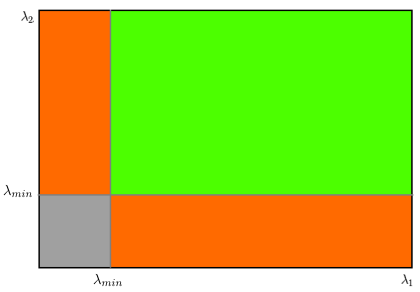
\includegraphics[width=0.75\textwidth]{figures/shitomasi_space.png}
	\caption{Image point classification based on Shi-Tomasi measure. Image source: OpenCV documentation}
	\label{fig:shiTomasiMeasure}
\end{figure}

Note that $M$ describes the shape of the local autocorrelation function's shape at the origin.
To describe $E$, \cite{Harris88alvey} uses the eigenvalues of the matrix $M$, as it provides a rotationally invariant description.
With this new method, the above mentioned cases (flat region, edge, corner) can be expressed as follows.
\begin{enumerate}
	\item \textbf{Flat region:} Both eigenvalues are small.
	\item \textbf{Edge region:} One eigenvalue of $M$ is small, the other is comparatively large.
	\item \textbf{Corner region:} Both eigenvalues are large.
\end{enumerate}
Figure \figref{harrisMeasure} shows the above defined regions with respect to the eigenvalues ($\alpha$ and $\beta$ are the eigenvalues of $M$).
The Harris detector also uses a metric for the "quality" of the detected edges or corners.
This is noted with $R$ and is defined below.
% Harris Measure
\begin{equation}
R = \det(M) - k(Trace(M))^2
\end{equation}
$k$ is a tunable parameter, its value is usually in the range of $0.01-0.05$.
The higher $R$ is, the more likely that a corner is present in the sampled window.
In figure \figref{harrisMeasure} the curves mark the regions in the $\alpha-\beta$ space that have the same $R$ value.

This is the short theoretical summary of the Harris detector.
A detailed mathematical derivation of the formulae can be found in \cite{Harris88alvey}.

The other corner detection method provided by the OpenCV framework is the Shi-Tomasi detector\cite{Shi94goodfeatures}.
This detector uses the same concept as the Harris detector, however uses a different measure to classify features as corners.
The scoring function is defined in \eqref{shiTomasiMeasure}. $\lambda_1, \lambda_2$ is the same as $\alpha, \beta$ for the Harris detector.
% Shi-Tomasi measure
\begin{equation}
	R = \min(\lambda_1, \lambda_2)
	\label{eq:shiTomasiMeasure}
\end{equation}
A feature is classified as a corner if $R$ is greater than a threshold $\lambda_{min}$.
Figure \figref{shiTomasiMeasure} shows this relation in the $\lambda_1-\lambda_2$ space.
The Shi-Tomasi measure, while being simpler and requiring less computational power, shows better performance in images\cite{Shi94goodfeatures}.

%-----------------------------------------------------------------------------------------------
\section{Application for Quad Detection}
%-----------------------------------------------------------------------------------------------

In this section the practical application of the previously explained algorithms will be presented.
The detection methods described in the above section provide solutions for detecting geometric primitives.
Some additional processing is required to use them for identifying quads on an image and measuring their parameters.
The details of the additional logic differ from algorithm to algorithm.
The preprocessing steps, the conversion of geometric primitives to quads and the various other necessary tasks will be explained below.
For the sake of simplicity, the steps of quad detection will be shown using a pseudo-code notation.

The experimental part of this work was done in python.
The quad detector prototypes and the test framework was developed using the language.
This greatly influenced the design of the framework used for testing: object oriented design principles were followed.
The quad detection routines were encapsulated in \textit{quad detectors}, which in turn are represented as instances of a \textit{QuadDetector} class.
Each detection method had it's own class, derived from the common ancestor.
The implementation details of the classes will not be described in depth, as they are only part of the test framework.
Only the parts necessary to understand the test method will be shown.

Each implemented detector had, as a public interface, a function called \textit{detect\_quad(img)}, which required an image containing a single quad.
The test framework operated on this simple interface.
The pseudo-code blocks of the following subsections will show how each detection method implemented this interface function.

As mentioned above, the exact python implementations will not be discussed.
They are far from optimal and there is lots of room for improvement.
However, in order to be complete, they are published in the appendix.

%-----------------------------------------------------------------------------------------------
\subsection{LSD Quad Detector}
%-----------------------------------------------------------------------------------------------

This quad detection method is built around the LSD algorithm.
The OpenCV implementation is used, which provides additional improvements around the algorithm described in the theoretical overview.
Namely, the scale dependence is handled within OpenCV.
It is done by generating a Gaussian pyramid from the input image, with $N-1$ down-sampling and $N$ Gaussian blurring, resulting in $N$ layers (one for each octave).
The above described LSD algorithm is then ran on each layer to detect lines of multiple scales.

That being said, not much additional logic was necessary to build a quad detection solution.
The detection routine is summed up in the listing below.
\begin{lstlisting}
detect_quad(img):
  img = prepare_image(img)
  lines, widths, prec, nfa = LSD_detector.detect(img)
	
  # Both edges of some line segment found
  if count(lines) > 3:
    pairs = find_pairs(lines, widths)
    lines_merged = merge_pairs(pairs, widths)
  elif count(lines) == 3:
    lines_merged = lines
  # Detection failed
  else:
    return None
	
  corners, result = find_corners(lines_merged)
  if result == (BaseNotFound or IntersectionNotFound):
    # detection fail
    return None
	
  return Quad(scale_to_quad_space(corners))
\end{lstlisting}

This line detection algorithm requires very little preprocessing.
The only necessary step is converting the 3 channel input image to grayscale.
Noise filtering is not needed as it is "built in" to the underlying algorithms.
First, the Gaussian down-sampling provides a quite efficient protection against white noise, jagged image edges or JPEG artefacts.
Furthermore, the \textit{a-contrario} validation of the LSD algorithm also provides efficient noise suppression.

It is possible that the LSD detects both edges of a line.
In that case, they need to be merged.
This is done by looking for almost parallel lines which are close together.
The merged line segments are calculated by selecting the longer one of the two parallel segments.
Then it is offset by half of the width of the detected line.
The LSD algorithm is sensitive to the gradient direction, so the direction of the offset can be calculated.

After the duplicates have been dealt with, the corner coordinates of the quad need to be found.
In order to do this, the quad base has to be identified.
The identification begins with creating every possible combination of the three line segments.
Then the distance of the line segments is calculated for each pair.
The pair with the maximum distance contains the the quad \textit{arms}, and the remaining segment is the \textit{base}.
The inner quad corner coordinates are found by calculating the intersection of each \textbf{line} representing an \textins{arm} with the one \textbf{line} representing the \textit{base}.
The outer corners (the end of the arms not connecting to the base) are simply the endpoints of each arm \textbf{line segment} further from the base.
This corner detection method is shared by all quad detectors using some kind of line detection.

Finally the corner coordinates are normed by the image size.
This is done in order to store the quad parameters in a way that does not depend on the image size.

%-----------------------------------------------------------------------------------------------
\subsection{Hough-based Quad Detectors}
%-----------------------------------------------------------------------------------------------

There are two quad detectors based on variants of the well known Hough-transform.
One is based on the Standard Hough-transform, the other is based on the PPHT.
Both versions of the transforms were covered in the theoretical overview.
The two detectors share many implementation details, so the common parts will be discussed first.
The different aspects will be covered separately.

The general flow of the Hough-based detection algorithms is given by the following pseudo-code.
The different underlying line detection methods are hidden behind the \textit{find\_segments} function.
The separate implementations will be discussed later.
\begin{lstlisting}
detect_quad(img):
  img = prepare_image(img)
	
  line_segments, result = find_segments(img)
  if result == NoLinesDetected:
    # Detection fail
    return None
	
  if count(line_segments) < 3:
    # Detection fail
    return None
	
  corners, result = find_corners(line_segments)
  if result == (BaseNotFound or IntersectionNotFound):
    # Detection fail
    return None
	
  return Quad(scale_to_quad_space(corners))	
\end{lstlisting}

The detection process starts by preparing the input image for the Hough-transform.
This involves two steps.
First the image is converted to binary by applying a threshold to it.
From the binary image the skeleton of the feature is extracted.
For this a simple algorithm is used, based on morphological operations.

The line detection is carried out on the skeleton image.
The detectors return the detected line segments.
Then the corner extraction described with the LSD based detector is applied.

After this overview of the general detection algorithm, the specialised cases of the standard and probabilistic Hough transform will be described.

%-----------------------------------------------------------------------------------------------
\subsubsection{SHT Quad Detector}
%-----------------------------------------------------------------------------------------------

The Hough transform is used in the line segment detection step.
It's implementation is provided by the OpenCV framework, but there are some supporting logic to get useful output from the detected lines.
The OpenCV function \textit{HoughLines} returns lines, represented by the \textit{Rho-Theta} parameters described in the theoretical overview.
It is not an easy task produce only the wanted lines with the classical Hough transforms.
Based on the above points, the supporting logic has to do two things.
First, the relevant lines need to be selected, then the endpoints of the lines have to be determined.

The line extraction routine is described in pseudo-code below.
The resolution of the accumulator was set to 1 pixel for \textit{rho} and $1^\circ$ for \textit{theta}.
The threshold for detection is determined by the bounding box of the skeleton on the image, as it correlates with the length of lines expected to be found.
\begin{lstlisting}
find_lines(img):
  thresh = get_threshold(img)
  lines = HoughLines(skeleton, 1, pi / 180, thresh)
  if lines is None or count(lines) < 3:
    return NoLinesDetected

  if count(lines) > 3:
    lines = kmeans(lines, number_of_clusters=3)
	
  return lines
\end{lstlisting}
The problem of more than 3 lines found is handled as follows.
The lines returned by the transform are clustered by the k-means algorithm.
The cluster centers returned by k-means each correspond to the average of one of the 3 dominant line groups.

As for the creation of line segments from the lines, the following algorithm is used.
First, the pixel from the original image touched by the given line are collected.
Then, the longest continuous\footnote{that is, having a smaller gap than defined by the max\_line\_gap variable} range of non-zero pixels are marked as part of the line segment.
\begin{lstlisting}
find_segments(img):
  lines, result = find_lines(img)
  if result == NoLinesDetected:
    # Detection failed
    return result
	
  max_line_gap = min(bounding_box_size) / 2
  segments = empty_list
  for rho, theta in lines:
    line_points = get_line_points(rho, theta, img)
    segments.append(get_line_segment(line_points, max_line_gap)
	
  return segments
\end{lstlisting}
The two ends of the region os the so marked pixels represent the endpoints of the line segment.
Then a list of the found line segments is returned.

%-----------------------------------------------------------------------------------------------
\subsubsection{PHT Quad Detector}
%-----------------------------------------------------------------------------------------------

The probabilistic Hough transform implementation is also provided by the OpenCV framework.
It requires additional parameters, as it handles the line to line segment conversion internally.

The PHT-based implementation of \textit{find\_segment} is described by the following pseudo-code.
The threshold for detection is calculated from the feature bounding box similarly to the SHT-based detector, the only differenc is a scale factor.
\begin{lstlisting}
find_segments(img):
  thresh = get_threshold(img)
  min_line_length = min(bounding_box_size) / 4

  lines = HoughLinesP(img, 1, np.pi / 180, thresh, 
                      minLineLength=min_line_length, 
                      maxLineGap=min_line_length/2)
  if lines is None or count(lines) < 3:
    return NoLinesDetected

  if count(line_segments) > 3:
    line_segments = merge_segments(line_segments)
				
  return line_segments
\end{lstlisting}
For the minimal required line length a simple heuristic is given, also based on the bounding box.

This detection method also suffers from the problem of more than necessary lines detected.
It is solved by merging the line segments having similar slope.
The detected line segments are returned to the common part of the code for quad corner calculation.

%-----------------------------------------------------------------------------------------------
\subsection{Corner Quad Detector}
%-----------------------------------------------------------------------------------------------

The corner detection based algorithm is fundamentally different than it's line detection based alternatives.
It is also simpler, as there is no line segment to corners conversion.
This detection method also has 2 variants depending on which corner measure they use.
However, this is handled inside OpenCV, so the variants differ only in a passed parameter.

The detection method overview is shown below.
The image preprocessing involves only a conversion to grayscale.
This could be improved, but for the preliminary testing it wasn't necessary, as optimally generated images were used.
\begin{lstlisting}
detect_quad(img):
  img = prepare_image(img)
  corners = get_corners(gray, max_corner_count=6, 
                              quality_level=0.1, 
                              min_distance=2, 
                              methotd=shi_tomasi)
	
  if count(corners) < 4:
    # Detection failed
    return None
	
  if count(corners) > 4:
    corners = merge_corners(corners)
	 
  inner, outer, result = identify_points(corners)
  if result == (BaseNotFound or TypeError):
    # Detection failed
    return None
	
  corners = [outer[0], inner[0], inner[1], outer[1]]	
  return Quad(scale_to_quad_space(corners))
\end{lstlisting}

The corner detection function was provided by OpenCV.
As mentioned above, the scoring function can be set to either Harris or Shi-Tomasi.
Both were tried, but there was no noticeable difference in the quality of detection.
Thus, the Shi-Tomasi method is used, as it is more efficient computationally.
The maximum number of corners to detect was seto to 6: the 2 endpoints of the arms, and the inner and outer corners of the intersection of base and arms.

The usual error handling is also present here: if less than 4 corners are detected, detection failure is reported.
If more (up to 6) corners ar detected, corner merging is done.
This is necessary if both the inner and the outer corner of the base-arm intersection is detected.
Those are merged together to their average.
For now, always the 2 closest points are merged.

In order to create a quad, the corner points have to be identified as an inner (base-arm intersection) or outer (arm end) points.
To do this, the connectivity of the point pairs is examined.
The connectivity check is done by counting the non-zero pixels along the line segment between the two selected corner point.
The points with 2 neighbours are classified as inner points, the ones having only one neighbour are the outer points.

When this classification is done, the detection process is finished.
A quad is created from the scaled corner points.